\documentclass[12pt]{article}
\usepackage[utf8]{inputenc}
\usepackage{cite}
\usepackage[utf8]{inputenc}
\usepackage{graphicx}
\usepackage{amsmath}
\usepackage[margin=0.5in]{geometry}
\pagenumbering{gobble}
%\usepackage{geometry}
\usepackage{pdfpages}
\usepackage{xcolor}
\usepackage{todonotes}
\usepackage{amsmath,amsfonts,amssymb,amsthm,epsfig,epstopdf,titling,url,array}
\setcounter{secnumdepth}{4}
%\usepackage{enumerate}% http://ctan.org/pkg/enumerate
\title{Computational Model of Peri-Personal Space}
\author{Joan Reyero}
%\date{\today}


\bibliographystyle{apalike}
%\bibliography{bib}


\begin{document}

\maketitle

\section{Reinforcement learning models}

\subsection{Data exploration}

Before attempting to fit a model some data exploration was performed. Figure \ref{fig:2.1} shows the number of times each participant chose stimulus $A$, and the total number of rewards obtained. While participants who chose more times stimulus $A$ tend to have higher rewards, there is not a clear pattern observable in the figure. 

\begin{figure}[h!]
	\centering
	\hspace*{-0.6in}
	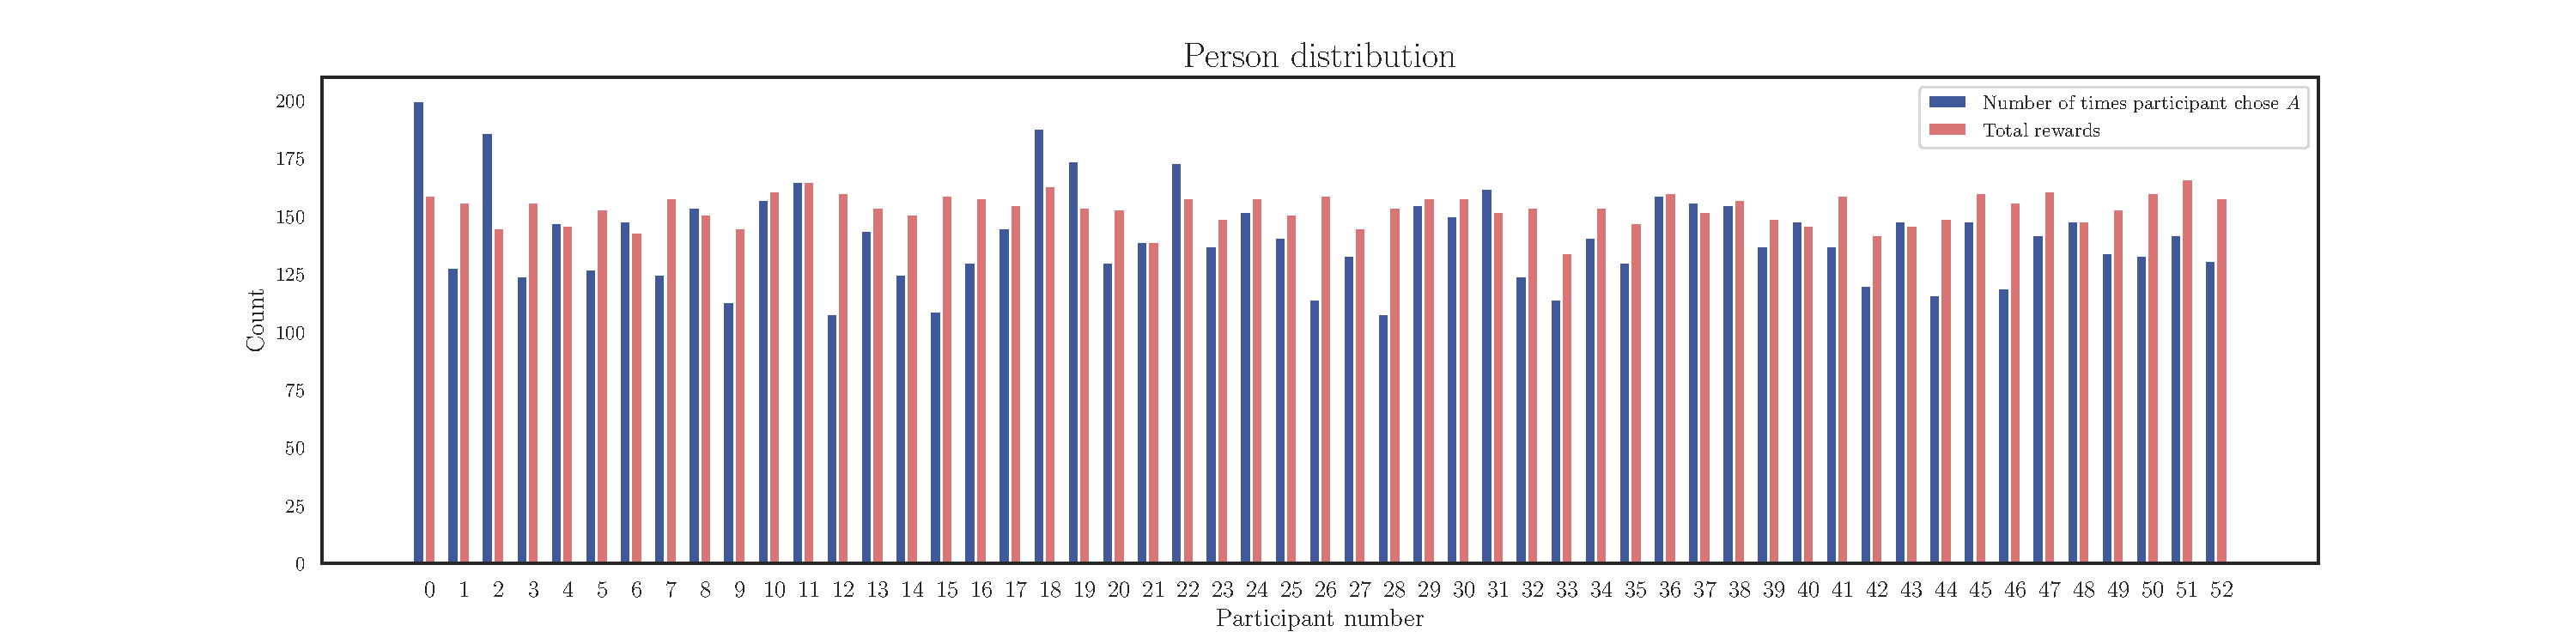
\includegraphics[width=1.2\linewidth]{figures/2.1.pdf}
	\caption{Plot of the total number of rewards and the number of times a participant chose stimulus $A$ for each participant.}
	\label{fig:2.1}
\end{figure}

The table below summarises the basic statistics for the studied variables. $A$ was chosen more than $50\%$ of the times, which is not surprising as, on average, choice $A$ had a higher probability of reward. The mean total rewards was 153.5, which is 64\% of the total.

The expected number of rewards if random choices were made can be obtained my

\[ \frac{\big(P(\mathrm{R} | A^1) + P(\mathrm{R} | B^1) + P(\mathrm{R} | A^2) + P(\mathrm{R} | B^2)\big) \times 100}{4} = 56.25 \]

Therefore, the expected number of rewards is lower than the average rewards obtained, which suggests that learning happened during the experiment.

\begin{center}
 \begin{tabular}{|c || c | c | c|} 
 \hline
  & Mean (out of 240) & Standard deviation & Range (out of 240) \\ [0.5ex] 
 \hline\hline
 Times $A$ was chosen & 141.0 & 20.31 & $[108, 200]$ \\ 
 \hline
 Total rewards & 153.5 & 6.63 & $[134,166]$ \\ [1ex] 
 \hline
\end{tabular}
\end{center}

\subsection{Simulated data exploration}

Figure \ref{fig:2.2} shows the average evolution of $V^A$, $V^B$ and $V^A - V^B$ for a simulation ran 100 times with 240 trials each. The trends clearly show that learning is happening with each probability switch, as when $V^A$ increases $V^B$ decreases and vice-versa. Moreover, it can be observer that when $P(\mathrm{R} | A) = 0.5 $ and $P(\mathrm{R} | B) = 0.75$ the learning happens slower than when $P(\mathrm{R} | A) = 0.75 $ and $P(\mathrm{R} | B) = 0.25$, as the difference in the probabilities is lower.

\begin{figure}[h!]
	\centering
	\hspace*{-0.4in}
	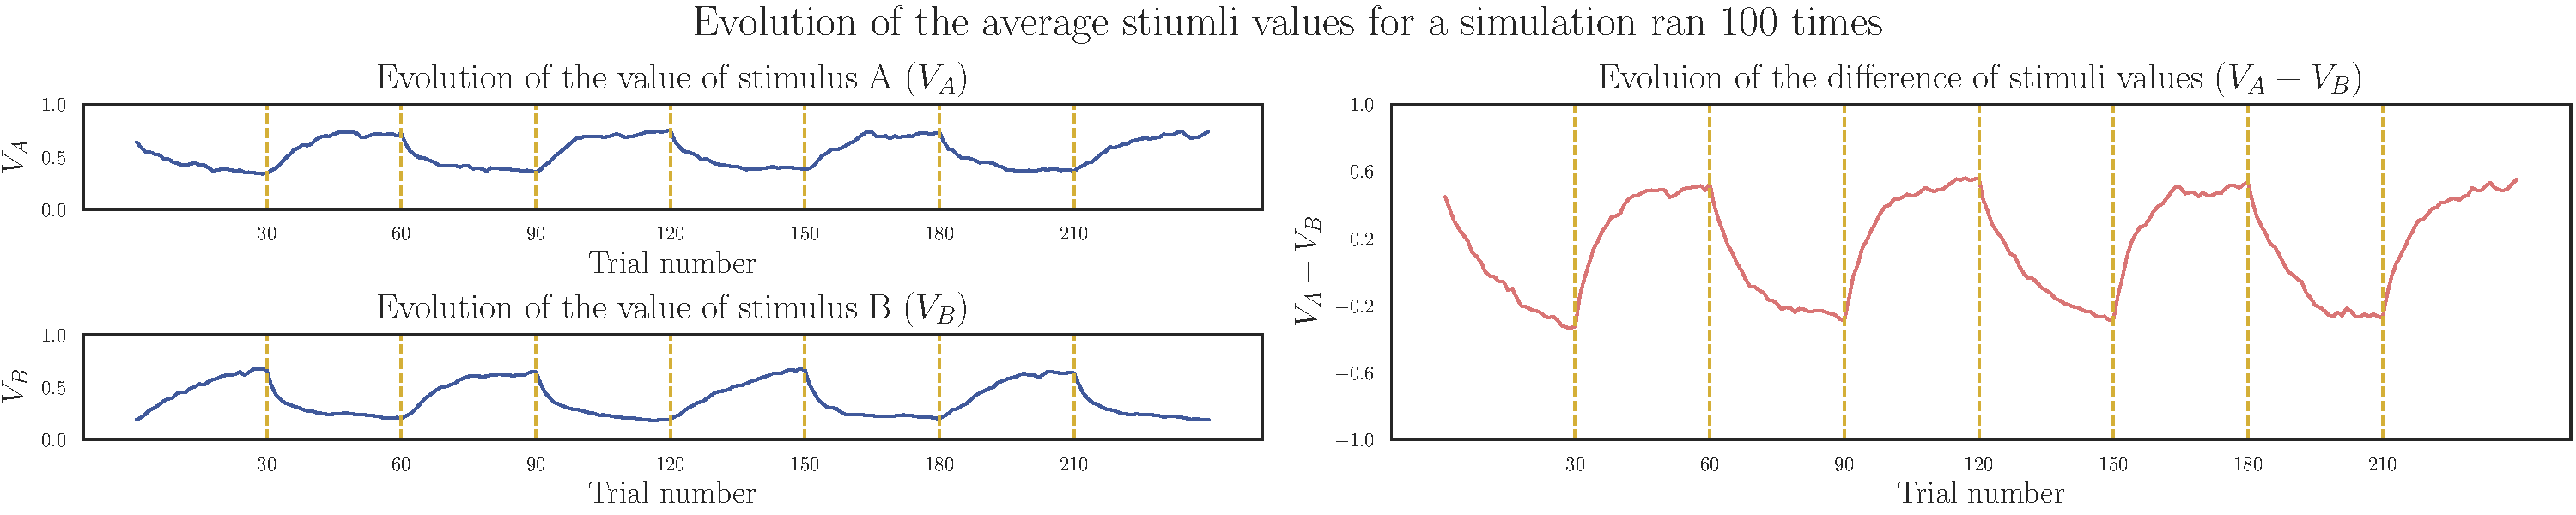
\includegraphics[width=1\linewidth]{figures/2.2.pdf}
	\caption{Plot of the average evolution of $V^A$ (top left), $V^B$ (bottom left) and $V^A - V^B$ (right), for a simulation ran 100 times with 240 trials. The golden dotted lines represent a switch in the probabilities.}
	\label{fig:2.2}
\end{figure}

The average number of rewards was 154.2.

\subsection{Parameter exploration}

For the parameter exploration, the values for the parameters were assigned:

\begin{description}
\item[$\epsilon_{\mathrm{values}}$:] linear space of 10 elements with range $[0, 1]$, 
\item[$\beta_{\mathrm{values}}$:] linear space of 15 elements with range $[1, 15]$.
\end{description}

Then, a simulation with 100 participants was performed for each pair of parameter values. 

\begin{figure}[h!]
	\centering
	\hspace*{-2.2in}
	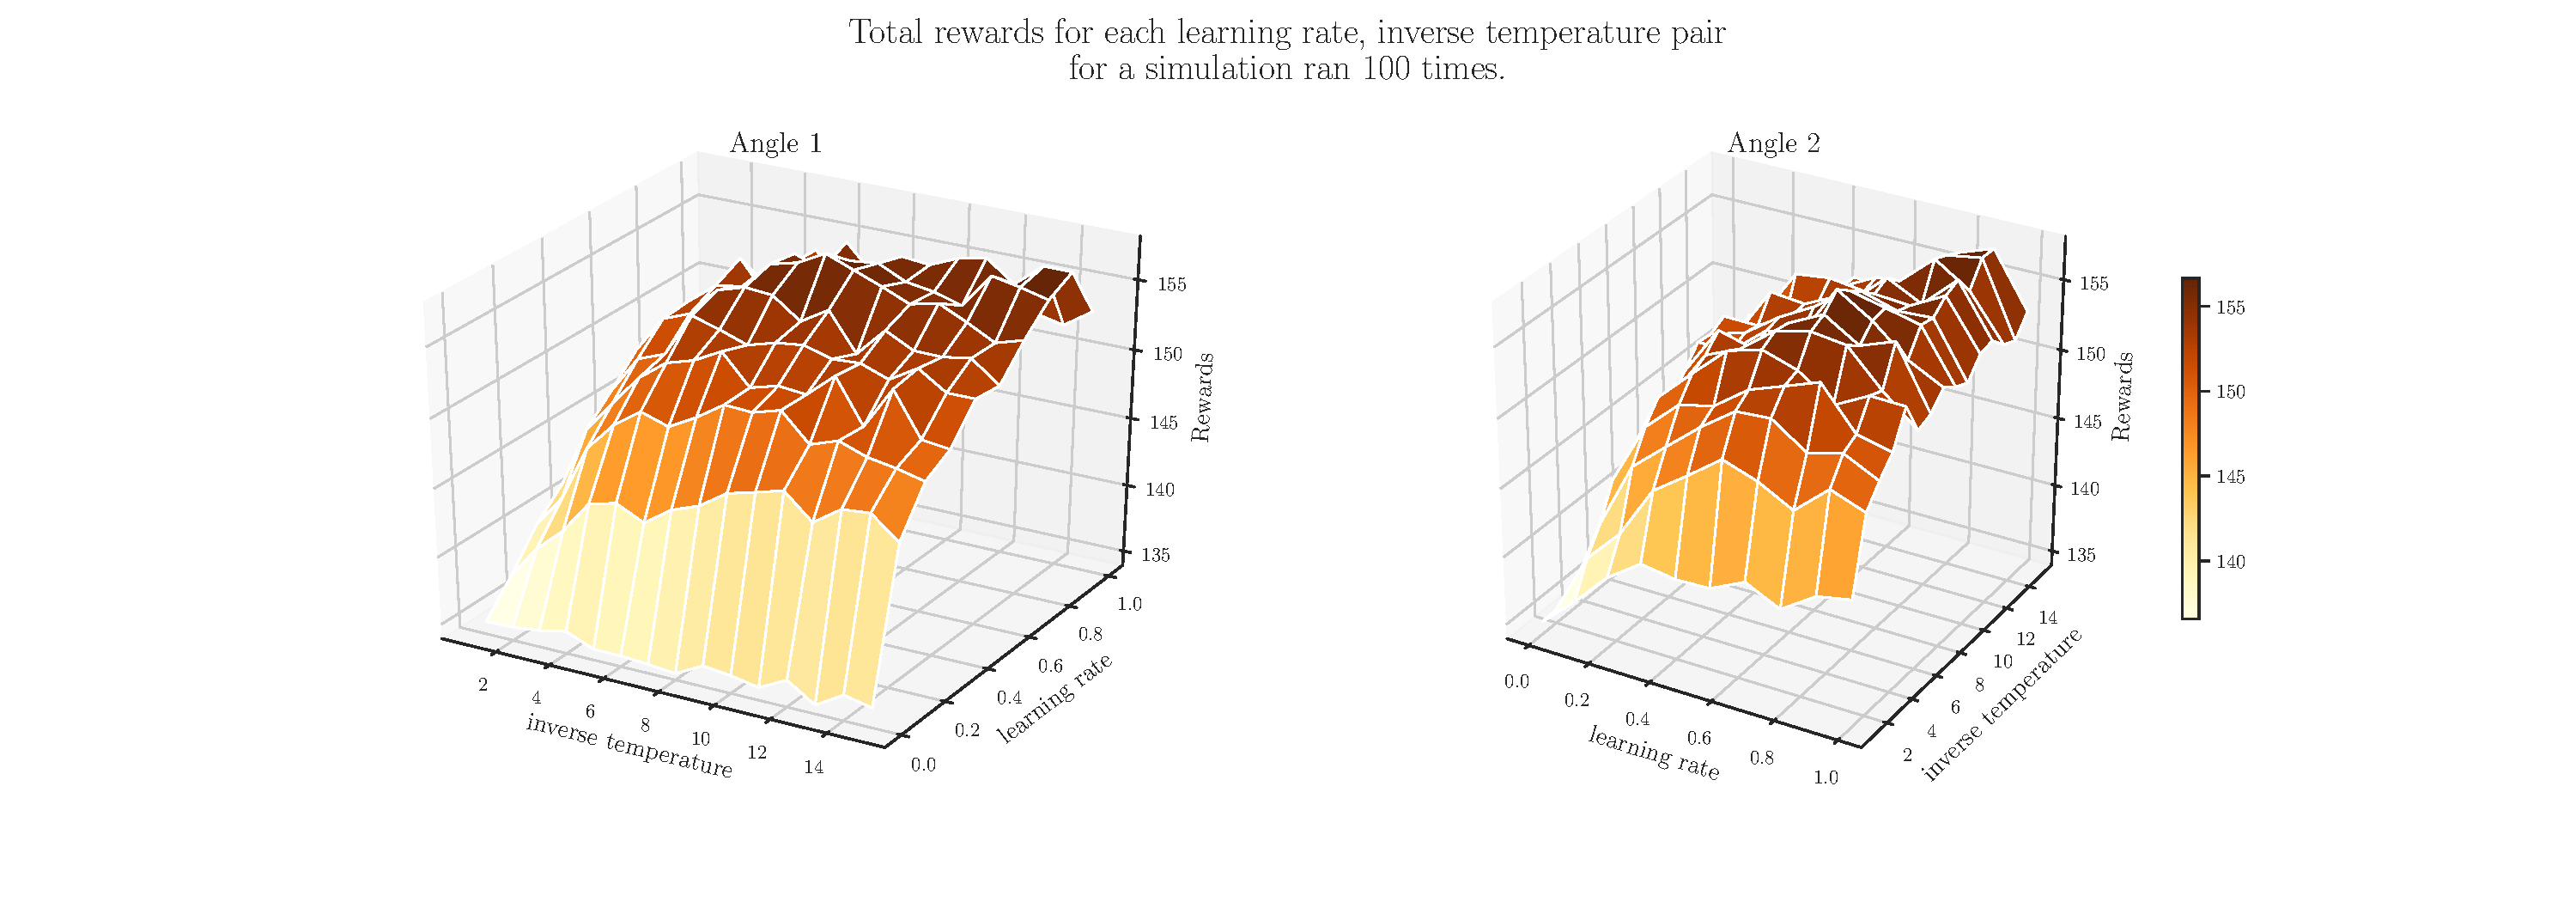
\includegraphics[width=1.5\linewidth]{figures/2.3.pdf}
	\caption{Plot of the number of rewards for each learning rate and negative energy pair. The two subplots correspond to two different angles to improve visibility.}
	\label{fig:2.3}
\end{figure}

Figure \ref{fig:2.3} shows the amount of reward of each pair of parameters. The reward increases as the negative energy increases from 0 to 10, and it stabilises afterwards. The learning rate also increases the reward as it increases up to a threshold of around 0.7, then the reward decreases as the learning rate increases.

\subsection{Negative log likelihood}

The negative log likelihood (NNL), using the formula provided in the report, was computed for the first participant, and it was 52 to two significant figures. 

For the second participant, the NNL was 63.83.

\subsection{Model fitting and group comparison}

\subsubsection{Model fitting}

The model was fit using the function \texttt{scipy.minimize} with the \texttt{BFGS} minimisation method \footnote{https://docs.scipy.org/doc/scipy/reference/generated/scipy.optimize.minimize.html}. $\epsilon = 0.5$ and $\beta = 5$ were used as starting parameters.

The minimisation algorithm encountered an overflow for most participants when running completely unconstrained. Therefore, the learning rate was constrained to being greater than 0, as there cannot be negative learning rates.

The mean learning rate (LR) found was 0.36, with a standard deviation of 0.123. The mean negative energy (NE) was 5.83, with a standard deviation of 1.25. 

\begin{figure}[h!]
	\centering
	\hspace*{-0.6in}
	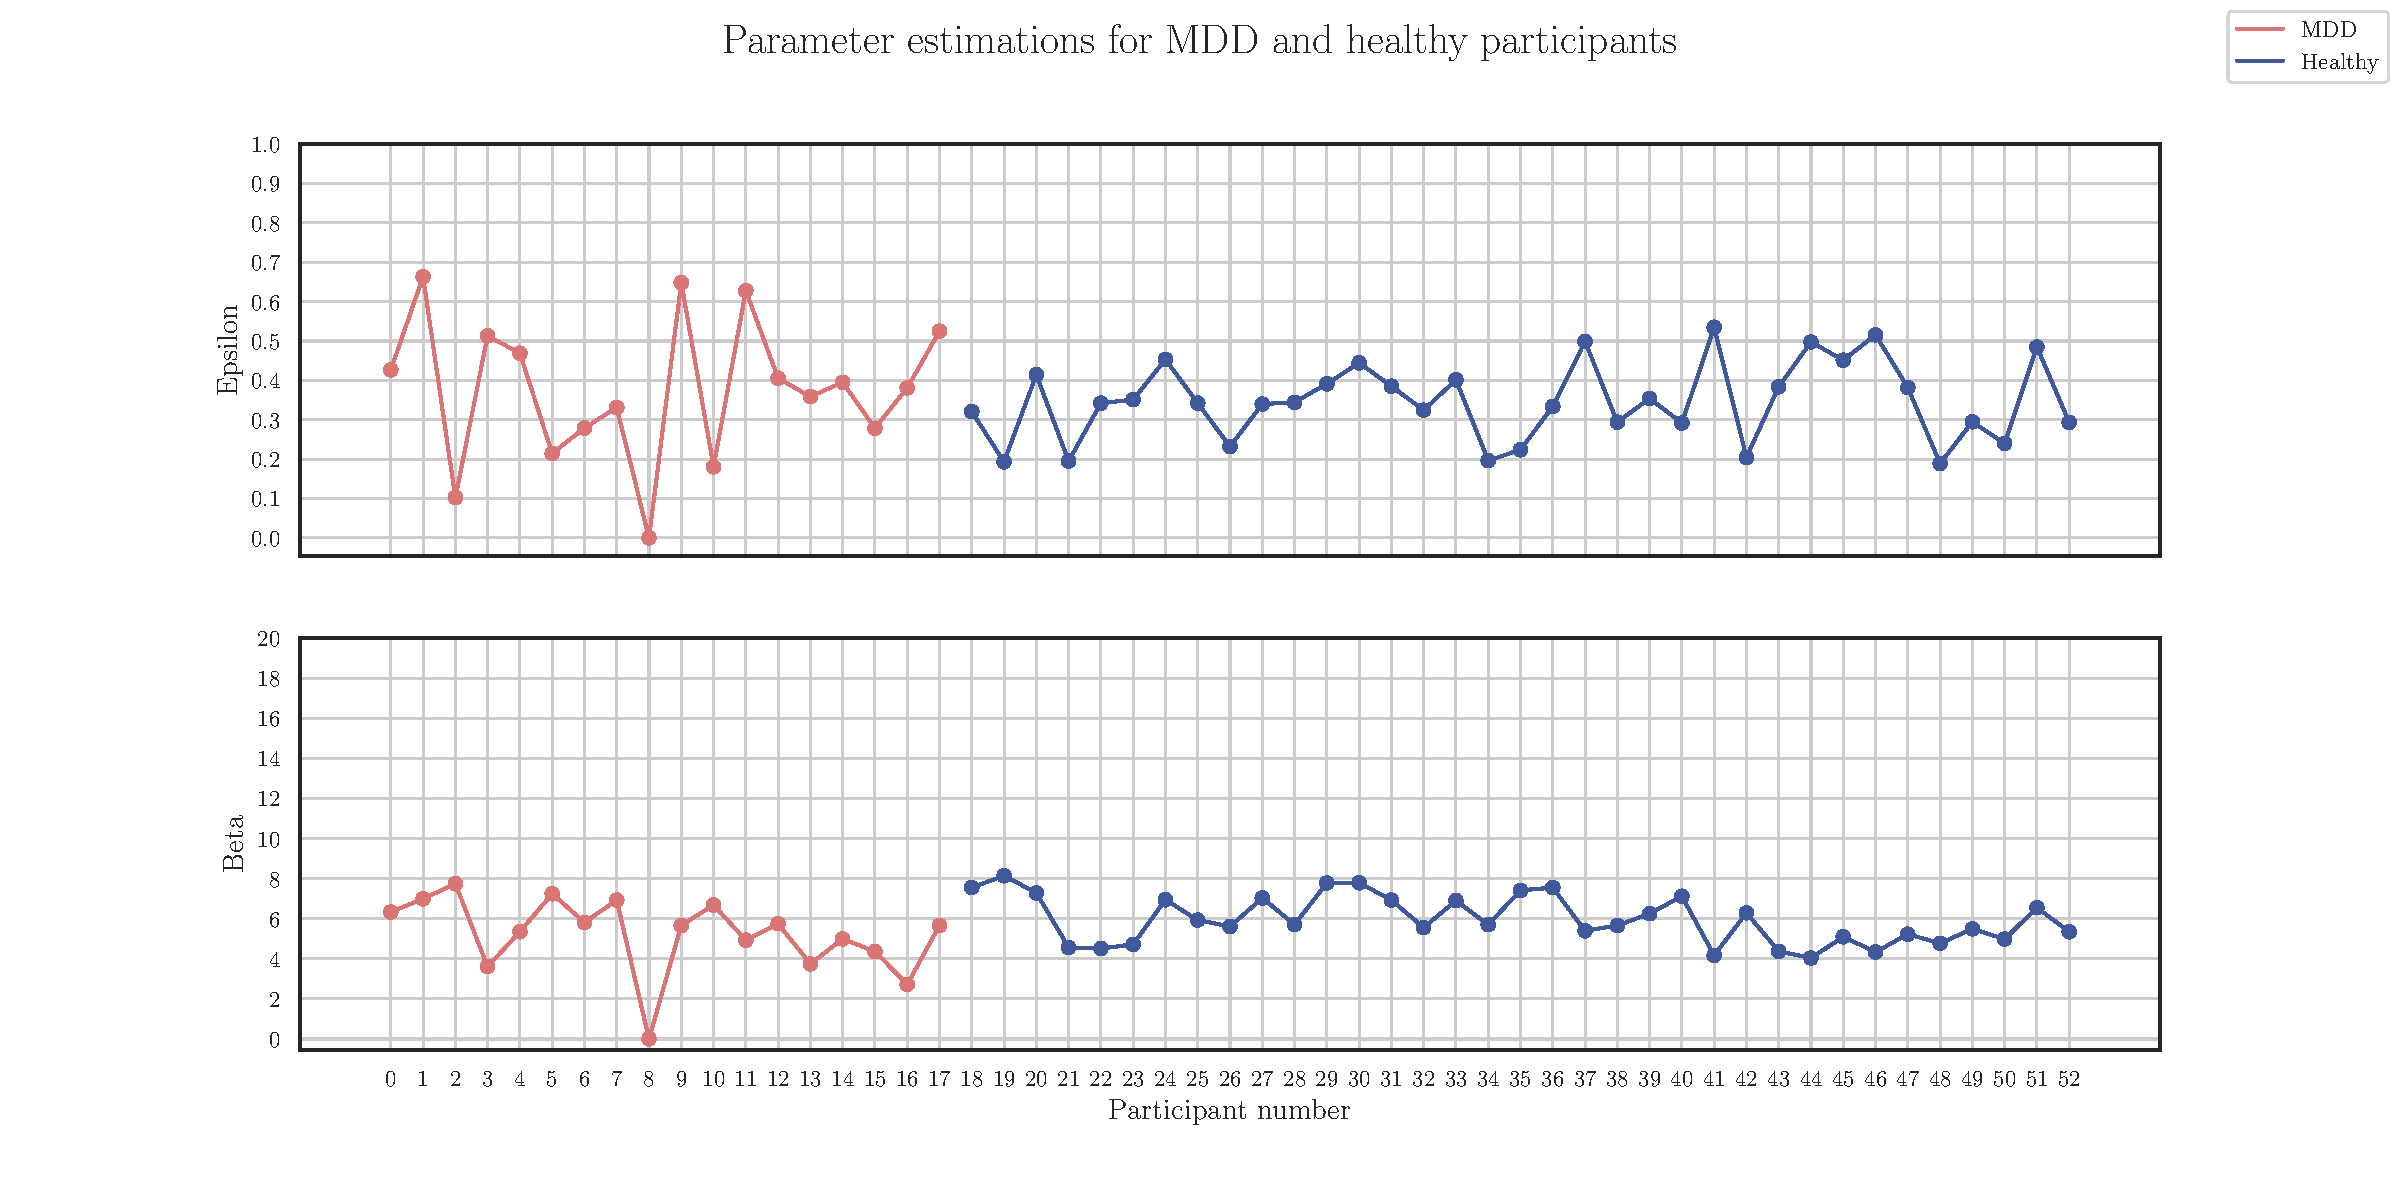
\includegraphics[width=1.2\linewidth]{figures/2.4.pdf}
	\caption{Best-fit learning rate (top) and negative energy (bottom) for healthy and MDD participants. The participants with 0 values were filtered-out because the best-fits were outside the normal range of $(0,1)$ for the LR and $(1, 15)$ for the NE.}
	\label{fig:2.4}
\end{figure}

Figure \ref{fig:2.4} shows the best-fit LR an NE for each participant, with considerably more variability in the MDD participants than in the healthy. It can also be observed that participant 8 has a value of 0 for both the LR and NE, this is because a filtering function was implemented to remove from the best-fit parameters those participants who did not fall within the normal range. The zero values seen in the plot are simply to keep the number of the participants constant, they were not taken into account for the reported statistics. 

Furthermore, the Pearson correlation coefficient was computed for all participants, and for the healthy and MDD participants together. The results can be seen in the table below. The p-value represents the probability that that the result would have been found if the correlation coefficient was 0.

\begin{center}
 \begin{tabular}{|c || c | c |} 
 \hline
  & Pearson correlation coefficient & p-value  \\ [0.5ex] 
 \hline\hline
 Overall & -0.22 & 0.11 \\ 
 \hline
 Healthy & -0.30 & 0.23 \\
 \hline
 MDD & -0.13 & 0.46 \\ [1ex] 
 \hline
\end{tabular}
\end{center}

There are no strong correlations between the best-fit LR and NE for any of the groups, which indicates that the optimisation algorithm functioned as expected, as high correlations would indicate anomalies in the data or the optimisation. 

\subsubsection{Group comparison}

A two-sample T-test between the healthy and MDD groups was performed for both the LR and the EPS. The null hypothesis was that $\mu_{\mathrm{healthy}} = \mu_{\mathrm{MDD}}$. The degrees of freedom in both cases were 16 (as only 17 MDD patients were considered). The results of the T-statistic and the p-value can be seen in the table below:

\begin{center}
 \begin{tabular}{|c || c | c |} 
 \hline
  & T-statistic & p-value  \\ [0.5ex] 
 \hline\hline
 LR & 1.33 & 0.19 \\
 \hline
 NE & -0.66 & 0.51 \\ [1ex] 
 \hline
\end{tabular}
\end{center}

There is only a 0.19 probability that the null hypothesis is true for the LR, therefore we can probably reject the null hypothesis and say that there is a difference between both means.

On the other hand, for the NE there is a 0.51 probability that the null hypothesis is true. Thus, we cannot accept nor reject the null hypothesis or establish a difference between groups.







\bibliography{bib}

\end{document}
